\chapter{Avaliação em Interação Humano-Computador}

\indent Atualmente a tecnologia está presente mais do que nunca em grande parte das atividades das pessoas, modernizando as casas, ruas, escolas, diferentes ambientes de trabalho, integrando-se na vida pessoal de cada um, se difundindo cada vez mais rápido. Estas tecnologias são chamadas TICs (Tecnologias da Informação e Comunicação) quando interferem direta e indiretamente nos processos de comunicação e informação dos indivíduos. 

\indent Para satisfazer certos critérios de qualidade, estes sistemas devem possuir algumas características que facilitem seu uso para seus usuários específicos. Ainda, vários métodos de avaliação podem ser aplicados sobre eles, cada um com um foco diferente a ser analisado. Em Ciência da Computação, a área de Interação Humano-Computador (IHC) é responsável por verificar a qualidade destes sistema mensurando certas propriedades e avaliar o impacto dos mesmos na vida dos usuários. 

\indent Na Seção \ref{IHC} serão descritos os conceitos básicos de IHC bem como os critérios de qualidade avaliados nas TICs. Na Seção \ref{avaObs} será apresentado um modelo de avaliação de sistemas computacionais, chamado Avaliação Através de Observação. Um método que utiliza este modelo, chamado Método de Avaliação de Comunicabilidade, será descrito detalhadamente também nessa seção e será utilizado neste projeto.
 
\section{Conceitos Básicos de IHC} \label{cbIHC}

\indent Esta seção apresenta os componentes básicos utilizados na matéria interdisciplinar Interação Humano-Computador, envolvidos na interação entre usuários e algum sistema computacional. A \textbf{interação} engloba todo o contato realizado pelo usuário com o objetivo de exercer uma tarefa através do sistema. Segundo John Kammersgaard, 1988, existem quatro perspectivas de interação usuário-sistema \cite{IHCbook}:
\begin{itemize}
\item[1] \textbf{Sistema}: Usuário conhece linguagem específica voltada para o sistema e seu objetivo é a transmissão correta dos dados da maneira mais rápida possível;
\item[2] \textbf{Parceiro de discurso}: Usuário interage com o sistema através de uma inteligência artificial que personifica um interlocutor especialista naquilo que usuário procura;
\item[3] \textbf{Mídia}: Usuários interagem entre si por meio do sistema, que pode oferecer diversos recursos como jogos e portal de notícias, porém é focado na qualidade da comunicação entre pessoas;
\item[4] \textbf{Ferramenta}: Usuário utiliza o sistema de maneira automática como instrumento de propósito geral para realizar suas tarefas. 
\end{itemize}

\indent Em um sistema interativo, a \textbf{interface} é responsável por manter o contato motor (como a \textit{webcam} e o teclado), perceptivo (como o monitor) e conceitual (interpretação do contato físico) do usuário \cite{IHCbook}. 

\indent O conjunto dos elementos da interface que expõem seu funcionamento de maneira implícita é chamado de \textbf{\textit{affordance}} \cite{IHCbook}. Esta palavra não possui tradução para o português, mas entende-se que significa "reconhecimento", pois uma vez que o usuário é levado a realizar os passos corretos para cumprir seus objetivos em uma interface, mesmo sem nunca ter interagido com ela antes, considera-se que ele já conhecia algumas características que o sistema oferece e obteve respostas já esperadas. Nesse sentido, a \textit{affordance} é geralmente uma característica muito desejável nos sistemas. Na Figura \ref{fig:Affordance} é possível perceber três graus diferentes de \textit{affordance} na \ref{fig:Affordance}.

\begin{figure}[!h]
    \centering
    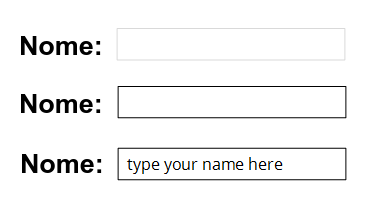
\includegraphics[width=0.4\textwidth]{affordance.png}
    \caption{Exemplo de tipos de caixa de texto que representam o mesmo campo (Nome) porém com níveis de \textit{affordance} diferentes, sendo que o último apresenta melhor o objetivo da caixa e, portanto, ela é reconhecida mais facilmente. Adaptado de \cite{affordance}.}
    \label{fig:Affordance}
\end{figure} 

\indent Em IHC, a qualidade de um certo sistema está fortemente relacionada à sua interface e interação \cite{IHCbook}, pois para que os usuários aproveitem o sistema por completo, eles deve estar confortáveis com o ambiente. As características da interação e interface que quantificam a qualidade de um sistema são chamadas de critérios de qualidade, apresentados a seguir:
\begin{itemize}
\item[1] \textbf{Usabilidade}: Medida de complexidade no aprendizado do uso da interface para atingir objetivos de maneira eficiente (no menor tempo possível, utilizando o menor número de recursos do sistema) e eficaz (de modo que o usuário execute as tarefas o mais automático possível, sem apresentar dúvidas a respeito da interface);
\item[2] \textbf{Experiência do usuário}: Medida de satisfação do usuário em relação ao sistema;
\item[3] \textbf{Acessibilidade}: Medida da flexibilidade do sistema, ou seja, da capacidade de usuários interagirem com o mesmo;
\item[4] \textbf{Comunicabilidade}: Medida da capacidade de transmissão das intenções do projetista do sistema para o usuário por meio da interface. %Exemplo: através de analogias
\end{itemize}

\indent Ao avaliar a qualidade de uso de um sistema, é necessário escolher um tipo de avaliação apropriado para o objeto estudado e para o critério de qualidade em foco, se existir. A avaliação através de inspeção, por exemplo, tenta conhecer as possíveis respostas do usuário em certas situação no sistema ainda em produção. Essa avaliação possui três métodos distintos, cada um com um objetivo diferente. O método pode ser heurístico (focada em problemas de usabilidade durante um processo interativo), cognitivo (focada em avaliar a facilidade de aprendizado de um sistema interativo) ou inspeção semiótica (focado em avaliar a quantidade de informação transmitida do projetista do sistema para o usuário).

\indent Outro tipo de avaliação bastante utilizado é o de avaliação por observação, o qual será utilizado neste trabalho. Esse tipo de avaliação considera problemas reais que os usuários (ou participantes com o mesmo perfil dos usuários) enfrenta ao utilizar o sistema. Existem três métodos de avaliação baseados em avaliação por observação: teste de usabilidade (focado em avaliar a usabilidade através de registros de performance e opiniões dos usuários), método de avaliação de comunicabilidade (focado em avaliar a quantidade de informação que chega ao usuário através do sistema) e prototipação em papel (focado em avaliar a usabilidade através de simulações do sistema em papel).  

\section{Avaliação Através de Observação} \label{avaObs}

\indent Para manter os critérios básicos de qualidades, é importante que exista algum tipo de avaliação do sistema antes de sua entrega ao(s) usuário(s). Na perspectiva de quem desenvolve o sistema, a avaliação deve verificar se o sistema recebe as entradas, processa os dados e gera o resultado na saída corretamente. Por outro lado, na perspectiva do usuário, a avaliação deve verificar como o comportamento da interface afeta a experiência de uso do sistema \cite{IHCbook}, recaindo nos quatro critérios de qualidade descritos na Seção \ref{cbIHC}. A etapa de avaliação pode ocorrer durante (\textbf{avaliação formativa}) ou após (\textbf{avaliação somativa}) o processo de desenvolvimento do sistema. Na primeira opção, o foco é a identificação de possíveis problemas, com a vantagem do baixo custo de correção. Na segunda opção, o foco é a verificação dos níveis de qualidade do protótipo de escopo definido \cite{IHCbook}.

\indent Os tópicos mais avaliados em IHC são os problemas na interação e na interface do sistema, que são classificados de acordo com a frequência com que ocorrem, com sua gravidade ou com os quatro critérios de qualidade. Um exemplo de questionário associado a esse tópico de avaliação encontra-se na parte de consolidação dos resultados, como será descrito a seguir nessa seção.

\indent A fundamentação dos métodos de avaliação é dada pela teoria da Engenharia Semiótica, focada em dois tipos de comunicações: usuário-sistema e projetista-usuário através do sistema. Esse último tipo de comunicação recebe o nome de \textbf{metacomunicação}, uma vez que é feita indiretamente através da interface criada pelo projetista para o usuário. Segundo esta teoria, toda aplicação computacional é um artefato de metacomunicação por onde o projetista, como interlocutor, comunica-se com o usuário. Quando o objetivo é avaliar a quantidade de emissão de metacomunicação, utiliza-se o Método de Inspeção Semiótica \cite{IHCbook}. Quando é avaliar a quantidade de recepção de metacomunicação, utiliza-se o Método de Avaliação de Comunicabilidade \cite{IHCbook}. 

\indent A \textbf{metamensagem} é a mensagem transmitida via metacomunicação. Em IHC, a metamensagem possui um padrão fixo e generalizado, que pode ser utilizado para facilitar o entendimento dos problemas do usuário, o que pode ser feito para solucioná-los e como fazê-lo. O texto a seguir representa esta mensagem e os campos entre os símbolos ``<'' e ``>'' representam um espaço a ser ocupado de acordo com o sistema desenvolvido:

\begin{quote}
Este é o meu entendimento, como \textit{<projetista do sistema>}, de quem você, \textit{<usuário específico / grupo de usuários>}, é, do que aprendi que você quer ou precisa \textit{<fazer / executar / visualizar / se comunicar>}, de que maneiras \textit{<prefere / é mais natural>} fazer, e \textit{<por quê / por quê não outras>}. O \textit{<nome do sistema>}, portanto, é o sistema que projetei para você, e \textit{<esta navegação específica>} é a forma como você pode ou deve utilizá-lo para alcançar uma gama de objetivos que se encaixam nesta visão.
\end{quote}

\indent A Semiótica também estuda a semiose: processo de significação dos signos, tudo o que é percebido pelos seres humanos e produz sensação, na mente dos intérpretes. Esse é um processo que transforma os fenômenos perceptíveis através dos sentidos em experiências dos indivíduos \cite{semiose01}. Analogamente, em IHC, a semiose é utilizada para compreender as ações tomadas, bem como as reações de resposta, pelos usuários que interagem com sistemas cobertos de signos. Nesse sentido, é possível elaborar um perfil semiótico do sistema para retratar os problemas de comunicabilidade, e, para isso, a metamensagem pode ser utilizada como base.


\subsection{Método de Avaliação de Comunicabilidade} \label{MAC}

\indent O Método de Avaliação de Comunicabilidade (MAC) é um método qualitativo de avaliação somativa, cujo objeto são os problemas na interação e interface do sistema, com foco na percepção do usuário. Ele consiste em uma análise de gravações em vídeo de pessoas utilizando o sistema com base em 13 etiquetas (expressões linguísticas que caracterizam ruptura na comunicação) e é composto por cinco etapas\cite{IHCbook}: preparação, coleta de dados, interpretação, consolidação dos resultados e relato dos resultados. As pessoas filmadas não são necessariamente os usuários do sistema, elas podem ser representantes de usuários que possuem o mesmo perfil daqueles para qual o sistema é direcionado. 

\subsubsection{Preparação}

\indent Nesta etapa, o avaliador é responsável por definir o perfil dos usuários, selecionar os representantes dos mesmos e elaborar o ambiente e tarefa realizada por eles. O material da gravação é preparado e verificado fazendo-se um teste piloto. Um termo de consentimento da avaliação deve ser redigido para assinarem o avaliador e cada representante. Devem ser elaborados dois questionários: um pré-teste, para coletar informações de cada representante tais como conhecimento sobre o domínio do sistema e um pós-teste, para coletar informações referentes à opinião dos participantes sobre suas experiências com o sistema.

\subsubsection{Coleta de Dados}

\indent Aqui o avaliador deve receber os representantes de usuários, explicar o procedimento da tarefa realizada, entregar uma via do termo de consentimento para cada representante assinar, já com a assinatura do avaliador. Os questionários pré-teste são entregues e cabe ao avaliador decidir se é necessário ler em voz alta as perguntas, caso alguma possa conter mais de uma interpretação. Não é especificado tempo mínimo nem máximo para esta tarefa. Ao final do questionário, o avaliador posiciona os equipamentos de gravação perto de cada participante, de maneira que a imagem gravada seja a tela, o \textit{mouse}/\textit{mousepad}, o teclado e as mãos dos mesmos, e o som captado seja apenas a voz dos mesmos. 

\indent Uma técnica muito conhecida de coleta de dados na gravação é chamada \textit{think aloud}, onde os participantes devem relatar em voz alta tudo aquilo que estão pensando em relação ao sistema, como execução, planejamento de execução, reação às respostas da interface, etc. O resultado final facilita bastante a análise do avaliador, porém o ato de falar enquanto desempenha a tarefa pode descentralizar o pensamento dos participantes. Uma vez que estes sintam-se seguros em realizar as tarefas ao mesmo tempo em que se expressam verbalmente, os avaliadores terão muito mais dados (etiquetas) para interpretar na fase seguinte.

\indent Terminada a gravação, ocorre uma entrevista para coletar a opinião de todos os participantes em relação ao sistema, bem como tirar dúvidas sobre seus desempenhos.

\subsubsection{Interpretação}

\indent Nesta etapa o avaliador assiste todos os vídeos contabilizando certas expressões linguísticas chamadas de etiquetas apresentadas na Tabela \ref{tabEtiquetas}. Deve-se levar em consideração os perfis dos usuários traçados pelo questionário pré-teste, bem como as entrevistas pós-teste, uma vez que as experiências passadas de cada um pode afetar seu comportamento no sistema. 

\indent As expressões linguísticas possuem na maioria conotação ruim com respeito ao sistema, tais como indagação sobre seu comportamento e aversão às respostas. Observando os vídeos, o avaliador pode perceber as barreiras de comunicabilidade e gargalos do sistema do ponto de vista do usuário, chamados de \textbf{falha de comunicabilidade}. Quando o número de participantes é muito baixo, o avaliador pode fazer a interpretação ao mesmo tempo em que coleta dados, sem precisar de gravação.

\begin{table}[]
\centering
\caption{Descrição das etiquetas, de acordo com a falha de comunicação que representam \cite{IHCbook}.}
\label{tabEtiquetas}
\begin{tabular}{|l|l|c|}
\hline
\multicolumn{3}{|l|}{\cellcolor[HTML]{9B9B9B}\specialcell{\textbf{Falhas de comunicação completas: efeito obtido é inconsistente com}\\\textbf{a intenção comunicativa do usuário}}} \\\hline
\textbf{aspecto semiótico}  & \textbf{característica específica} & \textbf{etiqueta} \\ \hline
\multirow{-2}{*}{\specialcell{O usuário termina uma\\semiose malsucedida,\\mas não inicia outra\\para obter o resultado\\esperado}}
    &  \specialcell{porque, mesmo percebendo que não obteve o\\resultado esperado, não possui mais recursos,\\capacidade ou vontade de continuar tentando}&Desisto \\ \cline{2-3} 
	&  \specialcell{porque não percebe que não obteve o\\resultado esperado}&\specialcell{Para mim\\está bom...} \\ \hline
		
		
\multicolumn{3}{|l|}{\cellcolor[HTML]{9B9B9B}\specialcell{\textbf{Falhas de comunicação parciais: o efeito obtido é somente parte do}\\\textbf{efeito pretendido de acordo com a intenção do usuário}}} \\ \hline
\textbf{aspecto semiótico}  & \textbf{característica específica} & \textbf{etiqueta} \\ \hline
\multirow{-2}{*}{\specialcell{O usuário abandona\\uma semiose antes de\\obter o resultado espe-\\rado, e inicia outra\\com o mesmo propósito}}
    & \specialcell{porque, embora entenda a solução de IHC\\proposta, prefere seguir por outro caminho no\\momento} & \specialcell{Não,\\obrigado} \\ \cline{2-3} 
    &  porque não entende a solução de IHC proposta & \specialcell{Vai de\\outro\\jeito}  \\ \hline

    
\multicolumn{3}{|l|}{\cellcolor[HTML]{9B9B9B}\specialcell{\textbf{Falhas de comunicação temporárias: o efeito parcial do processo de}\\\textbf{interpretação (semiose) e de comunicação (interação) do usuário é}\\\textbf{inconsistente e incoerente com sua intenção de comunicação}}}   \\ \hline
\textbf{aspecto semiótico}  & \textbf{característica específica} & \textbf{etiqueta} \\ \hline

\multirow{3}{*}{\specialcell{O usuário interrompe\\temporariamente sua\\semiose}}
   &\specialcell{porque não encontra uma expressão\\apropriada para sua intenção de comunicação}& Cadê?\\ \cline{2-3} 
   &\specialcell{porque não percebe ou não entende a\\expressão do sistema (preposto do projetista)}& \specialcell{Ué, o que\\houve?} \\ \cline{2-3} 
   &\specialcell{porque não consegue formular sua próxima\\intenção de comunicação}& E agora? \\ \hline
   
\multirow{3}{*}{\specialcell{O usuário percebe que\\seu ato comunicativo\\não foi bem-sucedido}}
   &\specialcell{porque percebeu que havia "falado" algo no\\contexto errado}&\specialcell{Onde\\estou?} \\ \cline{2-3} 
   & porque percebeu que havia "falado" algo errado & Epa!\\ \cline{2-3} 
   &\specialcell{porque não obteve o resultado esperado depois\\de conversar com o sistema (preposto do\\projetista) por algum tempo, alternando vários\\turnos de fala com ele}&\specialcell{Assim não\\dá.}\\ \hline
   
\multirow{4}{*}{\specialcell{O usuário procura com-\\preender o ato comuni-\\cativo do sistema\\(preposto do projetista)}}
   &através da metacomunicação implícita & \specialcell{O que é\\isto?}\\ \cline{2-3} 
   &através da metacomunicação explícita & Socorro!\\ \cline{2-3} 
   &\specialcell{testando várias hipóteses sobre o significado do\\que o sistema comunicou}&\specialcell{Por que\\não\\funciona?} \\ \hline   
\end{tabular}
\end{table}



\indent Após a análise dos dados, o avaliador deve redefinir um protótipo da próxima versão do sistema já com a solução para os problemas mais simples e listar todos os obstáculos na interface que podem ser corrigidos.


\subsubsection{Consolidação dos Resultados}

\indent Este é o momento em que o avaliador busca diferenciar as características do grupo das características individuais observando a recorrência das etiquetas em certos pontos da navegação no sistema. Pode-se atribuir significado às etiquetas de acordo com frequência de uso em um certo contexto, com sequência de uso e com o nível de problemas, por exemplo. Além disso, como o foco desta avaliação é verificar os problemas relacionados à interação e interface, nesta epata devem ser respondidas as seguintes questões:
\begin{itemize}
\item O usuário consegue operar o sistema?
\item Ele atinge seu objetivo? Com quanta eficiência? Em quanto tempo? Após cometer quantos erros?
\item Que parte da interface e da interação o deixa insatisfeito?
\item Que parte da interface o desmotiva a explorar novas funcionalidades?
\item Ele entende o que significa e para que serve cada elemento da interface?
\item Ele vai entender o que deve fazer em seguida?
\item Que problemas de IHC dificultam ou impedem o usuário de alcançar seus objetivos?
\item Onde esses problemas se manifestam? Com que frequência tendem a ocorrer? Qual é a gravidade desses problemas?
\item Quais barreiras o usuário encontra para atingir seus objetivos?
\item Ele tem acesso a todas as informações oferecidas pelo sistema?
\end{itemize} 

\indent Respondidas as perguntas, o avaliador pode criar então um perfil semiótico para o sistema com base na metamensagem a seguir:

\begin{quote}
Este é o meu entendimento, como projetista, de \textbf{quem você, usuário, é} (1), do que aprendi que você \textbf{quer ou precisa fazer} (2), de \textbf{que maneiras prefere fazer} (3), e \textbf{por quê} (4). Este, portanto, é o sistema que projetei para você, e esta é \textbf{a forma como você pode ou deve utilizá-lo} (5) para alcançar uma gama de objetivos que se encaixam nesta visão.
\end{quote}

\indent Cada item numerado na meta mensagem deve fornecer as seguintes informações buscadas:

\begin{itemize}
\item[(1)] Qual é o perfil dos usuários?
\item[(2)] Quais são seus desejos e o que a metacomunicação realiza para satisfazê-los?
\item[(3)] Quais as maneiras de realizar seus desejos e de que maneira eles preferem fazer?
\item[(4)] O que os leva a ter esta preferência?
\item[(5)] Quão bem o conteúdo da metacomunicação é transmitidos aos usuários?
\end{itemize}


\subsubsection{Relato dos Resultados}

\indent Ao final, o avaliador terá apresentar aos \textit{stakeholders} responsáveis pelo desenvolvimento do sistema os seguintes resultados:

\begin{itemize}
\item Os objetos da avaliação;
\item Breve descrição do método de avaliação;
\item Número e perfil dos avaliadores e representantes de usuários;
\item Descrição das tarefas executadas pelos participantes;
\item Resultado das etiquetagens, em geral contabilizando as etiquetas por usuário e tarefa;
\item Problemas de comunicabilidade encontrados;
\item Sugestões de melhoria;
\item Perfil semiótico do sistema.
\end{itemize}


%http://acervodigital.ufpr.br/bitstream/handle/1884/36666/Luiz%20Augusto%20Sakakibara.pdf?sequence=1


